\begin{figure}[htbp]
\centering
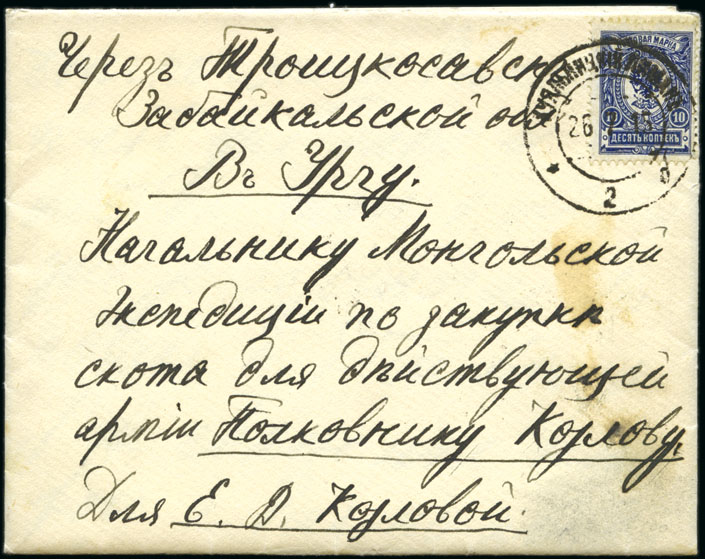
\includegraphics[width=.95\textwidth]{../russian-post-in-mongolia/10145.jpg}
\caption{ 
10145 URGA INCOMING: 1915 Envelope from Kuyanitsyi Liman (near Odessa) 
to Colonel Kozlov, Head of the Mongolian Expedition to Purchase Cattle 
for the Russian Army in Urga (and famous Russian explorer) for transmission
to a relative, franked with 10k blue, Troitskosavsk and Urga type 7A bs,
including contents, fine and rare incoming mail.
\euro 300.00 
} 
\end{figure}  

\begin{figure}[htbp]
\centering
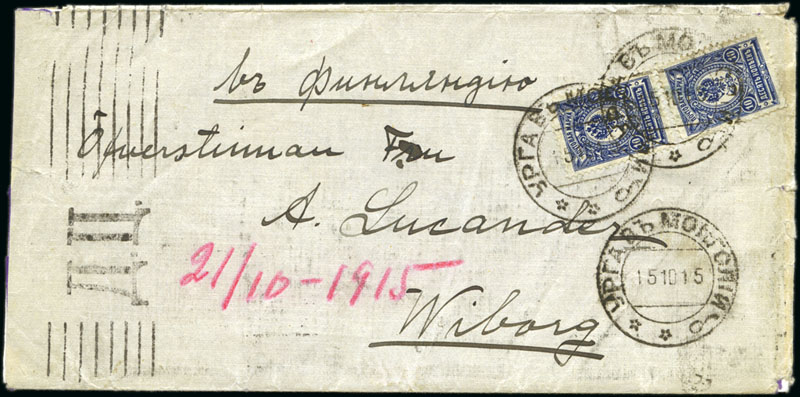
\includegraphics[width=.95\textwidth]{../russian-post-in-mongolia/10146.jpg}
\caption{ 
10146	URGA: 1915 Envelope to Viborg, Finland, franked with two 10k
blue paying double the 10k letter rate, tied by Urga 15.10.15 type 7A cds,
with Finnish censor mark at left, fine and uncommon destination.
\euro400.00 
} 
\end{figure}  

\begin{figure}[htbp]
\centering
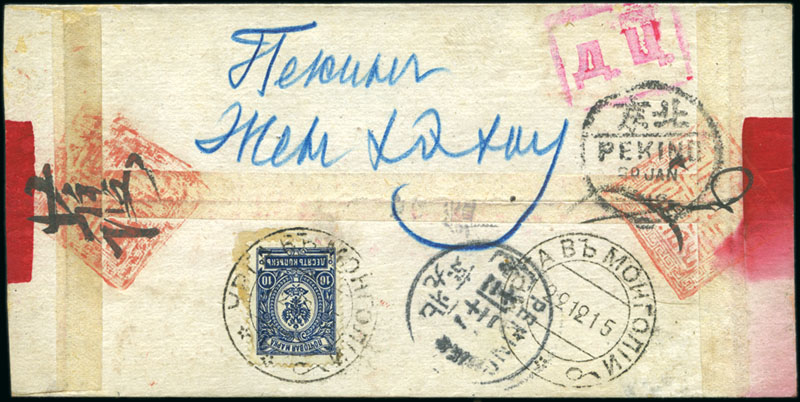
\includegraphics[width=.95\textwidth]{../russian-post-in-mongolia/10147.jpg}
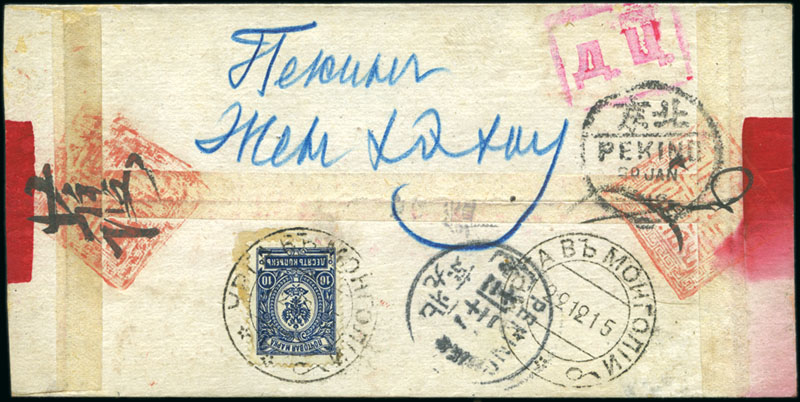
\includegraphics[width=.95\textwidth]{../russian-post-in-mongolia/10147.jpg}
\caption{ 
10147 URGA: 1915 Native cover to Peking, franked with 1909-12 10k blue 
paying the single rate, tied by Urga 22.12.15 type 7A cds, with Chinese 
P.O. Peking transits and Russian censor mark applied at Manchuli, very fine
\euro 300.00 
} 
\end{figure}  

\begin{figure}[htbp]
\centering
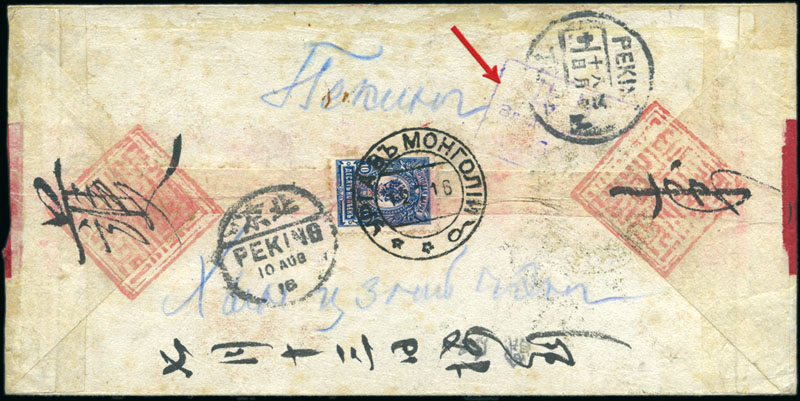
\includegraphics[width=.95\textwidth]{../russian-post-in-mongolia/10148.jpg}
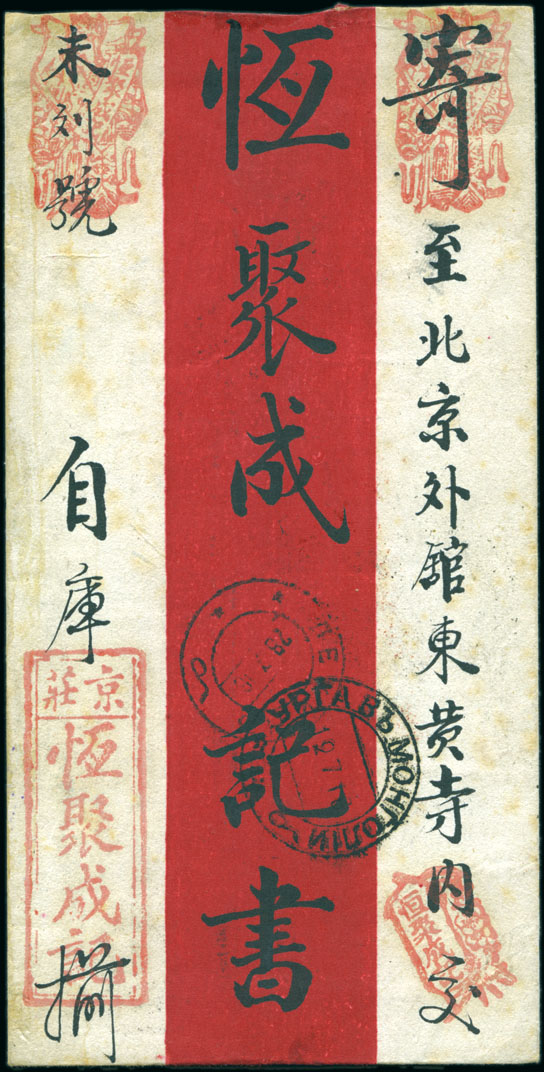
\includegraphics[width=.50\textwidth]{../russian-post-in-mongolia/10148-1.jpg}
\caption{ 
10148	URGA: 1916 Native cover to Peking, franked with 10k blue paying
single rate, tied by Urga 12.7.16 type 7A cds, with Russian and Chinese 
Peking arrival ds and violet censor hs from Vladivostok, fine
\euro 300.00 
} 
\end{figure}  

\section{Value Declared}

\begin{figure}[htbp]
\centering
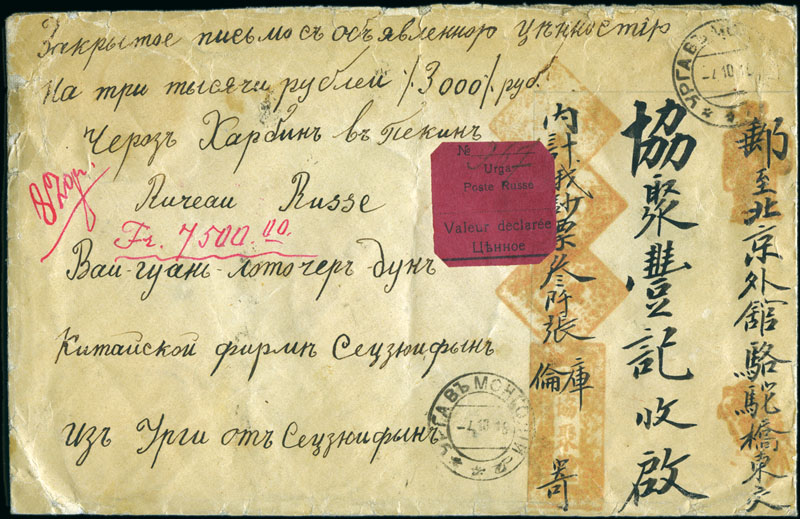
\includegraphics[width=.95\textwidth]{../russian-post-in-mongolia/10149.jpg}
\caption{ 
10149	URGA: 1916 "Value Declared" envelope for 3'000R to Peking,
franked on the reverse with 1909-12 1k, 35k, 50k and 1R pair, tied by
Urga 4.10.16 type 7A cds, obverse with red "Urga / Poste Russe / 
Valuer delcar\'ee" label (Hellrigl type 1 rated RRR, one of two known examples, 
sent via the Russian P.O. at Harbin and the Japanese P.O. at Changchun
\euro 3,000.00.
} 
\end{figure}

Lorem ipsum dolor sit amet, consectetur adipiscing elit. Sed nibh justo, dictum sed cursus ac, lobortis et lacus. Vestibulum vitae justo enim. Quisque laoreet elementum felis, ut sodales arcu viverra a. Sed molestie odio vulputate sem rutrum a sagittis est rutrum. Morbi dapibus hendrerit magna, sit amet commodo massa posuere sit amet. Duis pharetra quam scelerisque est lobortis fringilla. Maecenas venenatis feugiat lectus, vel facilisis odio pharetra quis. Etiam at nisl eros, sit amet suscipit lorem. Lorem ipsum dolor sit amet, consectetur adipiscing elit. Sed augue nunc, ornare eget congue sit amet, laoreet vel augue. Morbi vel justo quis ipsum adipiscing egestas vitae non est. Vivamus ac quam quam. Nullam pharetra
                                                    interdum mauris, rutrum pulvinar ligula condimentum id. Donec et blandit lorem. 




                        